% =============================================================================
% Phase 1 — Flow Network Formalization of the Mining Dynamic Routing System
% =============================================================================
% Grounded in the mining-drs codebase (drs_mining/components/).
% No individual vehicles are instantiated; the fleet is a distributed,
% continuous capacity flowing through a directed graph.
% =============================================================================

\documentclass[11pt,a4paper]{article}

% ── Packages ─────────────────────────────────────────────────────────────────
\usepackage[utf8]{inputenc}
\usepackage[T1]{fontenc}
\usepackage{amsmath,amssymb,amsthm}
\usepackage{mathtools}
\usepackage{booktabs}
\usepackage{longtable}
\usepackage{array}
\usepackage{geometry}
\usepackage{tikz}
\usetikzlibrary{arrows.meta,positioning,calc,decorations.markings,shapes.geometric}
\usepackage{hyperref}
\usepackage{cleveref}
\usepackage{enumitem}
\usepackage{xcolor}
\usepackage{float}

\geometry{margin=2.5cm}

\definecolor{sourceColor}{HTML}{2ca02c}
\definecolor{sinkColor}{HTML}{d62728}
\definecolor{intersectionColor}{HTML}{1f77b4}
\definecolor{stockpileColor}{HTML}{ff7f0e}

\newcommand{\tph}{\,\text{t/d}}                    % tonnes per day
\newcommand{\R}{\mathbb{R}}

\theoremstyle{definition}
\newtheorem{definition}{Definition}[section]
\newtheorem{constraint}{Constraint}[section]

\title{%
  \textbf{Phase 1: Flow Network Formalization}\\[6pt]
  \large Dynamic Routing System for Underground Mine Operations}
\author{Mining-DRS Project}
\date{\today}

\begin{document}
\maketitle
\tableofcontents
\newpage

% ═════════════════════════════════════════════════════════════════════════════
\section{Overview}
% ═════════════════════════════════════════════════════════════════════════════

This document formalizes the mining system implemented in the
\texttt{drs\_mining} codebase as a \emph{continuous, aggregate flow network}.
No individual truck objects, IDs, or stochastic travel times appear; the
fleet is treated as a distributed, fluid capacity.  The formalization maps
directly to the codebase's \texttt{ConcentratorConfig},
\texttt{MultiFaceConcentratorController}, \texttt{ContinuousFleetLogistics},
\texttt{ContinuousMineFace}, \texttt{Stockpile}, and
\texttt{ConcentratorPlant} modules.

The system is an underground base-metal flotation concentrator with:
\begin{itemize}[nosep]
  \item Two stochastic mining faces (Face~1 and Face~2), each producing ore
        with a different mean Ore-1 fraction.
  \item A fleet of LHDs (loaders) and haul trucks, continuously allocated
        across the faces.
  \item Two segregated stockpiles (Ore~1 and Ore~2) feeding a processing
        plant.
  \item A multi-mode blending controller that shifts between seven distinct
        operating modes.
\end{itemize}


% ═════════════════════════════════════════════════════════════════════════════
\section{Mine Topology: Directed Graph \texorpdfstring{$G = (V, E)$}{G = (V,E)}}
\label{sec:topology}
% ═════════════════════════════════════════════════════════════════════════════

\subsection{Node Definitions}

\begin{definition}[Graph Vertices]
$V = S \cup I \cup D$ where:
\begin{align}
  S &= \{s_1, s_2\}            && \text{Sources (mining faces)} \\
  I &= \{n_{\text{jct}}\}       && \text{Intersections (underground junction)} \\
  D &= \{d_{\sigma_1}, d_{\sigma_2}, d_p\}
                                 && \text{Sinks (Ore-1 stockpile, Ore-2 stockpile, plant discharge)}
\end{align}
\end{definition}

\noindent
\textbf{Node catalogue} (grounded in codebase entities):

\begin{table}[H]
\centering
\caption{Graph vertices and their physical correspondences.}
\label{tab:nodes}
\begin{tabular}{@{}llll@{}}
\toprule
\textbf{Symbol} & \textbf{Type} & \textbf{Code Entity} & \textbf{Description} \\
\midrule
$s_1$                & Source       & \texttt{ContinuousMineFace(face\_id=1)} & Face~1 ($\bar{g}_1 = 0.85$ ore-1 fraction) \\
$s_2$                & Source       & \texttt{ContinuousMineFace(face\_id=2)} & Face~2 ($\bar{g}_2 = 0.55$ ore-1 fraction) \\
$n_{\text{jct}}$     & Intersection & \texttt{ContinuousFleetLogistics}       & Underground junction / fleet merge point \\
$d_{\sigma_1}$       & Sink         & \texttt{Stockpile("Ore1Stock")}         & Ore-1 stockpile \\
$d_{\sigma_2}$       & Sink         & \texttt{Stockpile("Ore2Stock")}         & Ore-2 stockpile \\
$d_p$                & Sink         & \texttt{ConcentratorPlant}              & Processing plant (final discharge) \\
\bottomrule
\end{tabular}
\end{table}

\subsection{Edge Definitions}

\begin{definition}[Graph Edges]
$E = E_{\text{haul}} \cup E_{\text{route}} \cup E_{\text{process}}$ where each
edge $e = (i,j)$ carries physical attributes $(L_{ij}, V_{ij}^{\max})$:
\end{definition}

\begin{table}[H]
\centering
\caption{Directed edges with physical attributes (default configuration).}
\label{tab:edges}
\begin{tabular}{@{}lllrrl@{}}
\toprule
\textbf{Edge} & \textbf{From} & \textbf{To} & $L_{ij}$ \textbf{(km)} & $V_{ij}^{\max}$ \textbf{(km/h)} & \textbf{Category} \\
\midrule
$e_1$ & $s_1$ & $n_{\text{jct}}$     & 1.5 & 15 & Haul (Face~1 $\to$ Junction) \\
$e_2$ & $s_2$ & $n_{\text{jct}}$     & 2.2 & 15 & Haul (Face~2 $\to$ Junction) \\
$e_3$ & $n_{\text{jct}}$ & $d_{\sigma_1}$ & 0   & $\infty$ & Routing (logical split to Ore-1 pile) \\
$e_4$ & $n_{\text{jct}}$ & $d_{\sigma_2}$ & 0   & $\infty$ & Routing (logical split to Ore-2 pile) \\
$e_5$ & $d_{\sigma_1}$ & $d_p$         & 0   & $\infty$ & Process (stockpile$\to$plant feed) \\
$e_6$ & $d_{\sigma_2}$ & $d_p$         & 0   & $\infty$ & Process (stockpile$\to$plant feed) \\
\bottomrule
\end{tabular}
\end{table}

\noindent
Edges $e_3$--$e_6$ are logical (zero-length); physical hauling only occurs on
$e_1$ and $e_2$.  Lengths come from \texttt{config.face\_haul\_distance = (1.5, 2.2)}.
Maximum speed is \texttt{config.truck\_velocity = 15} km/h.

\subsection{Graph Schematic}

\begin{figure}[H]
\centering
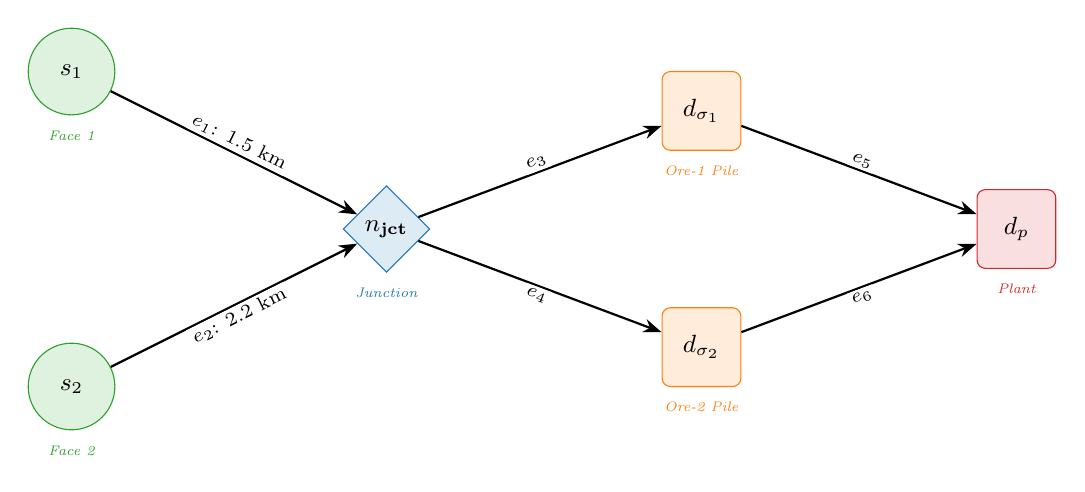
\begin{tikzpicture}[
    >=Stealth,
    source/.style={circle, draw=sourceColor, fill=sourceColor!15, minimum size=1.1cm, font=\small\bfseries},
    junction/.style={diamond, draw=intersectionColor, fill=intersectionColor!15, minimum size=1.1cm, font=\small\bfseries, inner sep=1pt},
    stockpile/.style={rectangle, draw=stockpileColor, fill=stockpileColor!15, minimum size=1.0cm, font=\small\bfseries, rounded corners=3pt},
    plant/.style={rectangle, draw=sinkColor, fill=sinkColor!15, minimum size=1.0cm, font=\small\bfseries, rounded corners=3pt},
    edgelabel/.style={font=\scriptsize, fill=white, inner sep=1pt},
  ]

  % Nodes
  \node[source]    (s1) at (0, 2)   {$s_1$};
  \node[source]    (s2) at (0,-2)   {$s_2$};
  \node[junction]  (jct) at (4, 0)  {$n_{\text{jct}}$};
  \node[stockpile] (sp1) at (8, 1.5) {$d_{\sigma_1}$};
  \node[stockpile] (sp2) at (8,-1.5) {$d_{\sigma_2}$};
  \node[plant]     (plt) at (12, 0)  {$d_p$};

  % Labels beneath nodes
  \node[below=2pt, font=\tiny\itshape, text=sourceColor] at (s1.south) {Face 1};
  \node[below=2pt, font=\tiny\itshape, text=sourceColor] at (s2.south) {Face 2};
  \node[below=2pt, font=\tiny\itshape, text=intersectionColor] at (jct.south) {Junction};
  \node[below=2pt, font=\tiny\itshape, text=stockpileColor] at (sp1.south) {Ore-1 Pile};
  \node[below=2pt, font=\tiny\itshape, text=stockpileColor] at (sp2.south) {Ore-2 Pile};
  \node[below=2pt, font=\tiny\itshape, text=sinkColor] at (plt.south) {Plant};

  % Edges
  \draw[->, thick] (s1) -- node[edgelabel, above, sloped] {$e_1$: 1.5 km} (jct);
  \draw[->, thick] (s2) -- node[edgelabel, below, sloped] {$e_2$: 2.2 km} (jct);
  \draw[->, thick] (jct) -- node[edgelabel, above, sloped] {$e_3$} (sp1);
  \draw[->, thick] (jct) -- node[edgelabel, below, sloped] {$e_4$} (sp2);
  \draw[->, thick] (sp1) -- node[edgelabel, above, sloped] {$e_5$} (plt);
  \draw[->, thick] (sp2) -- node[edgelabel, below, sloped] {$e_6$} (plt);

\end{tikzpicture}
\caption{Directed graph $G=(V,E)$ of the baseline two-face underground mine.
Sources are circles (\textcolor{sourceColor}{green}),
the junction is a diamond (\textcolor{intersectionColor}{blue}),
stockpiles are rounded rectangles (\textcolor{stockpileColor}{orange}),
and the plant is a rounded rectangle (\textcolor{sinkColor}{red}).}
\label{fig:graph}
\end{figure}


% ═════════════════════════════════════════════════════════════════════════════
\section{Macro-State Variables}
\label{sec:variables}
% ═════════════════════════════════════════════════════════════════════════════

All variables are continuous functions of time $t$.  No vehicle indices appear.

\subsection{Edge Flow Variables}

\begin{definition}[Flow Rate]
For each edge $(i,j) \in E$, the \emph{flow rate} $Q_{ij}(t)$ is the mass of
material traversing the edge per unit time (tonnes/day).
\end{definition}

\begin{center}
\begin{tabular}{@{}llp{8cm}@{}}
\toprule
\textbf{Symbol} & \textbf{Edge} & \textbf{Description} \\
\midrule
$Q_{s_1, n}(t)$ & $e_1$ & Total extraction rate from Face~1 (maps to \texttt{face\_achieved\_extraction\_rates[0]}) \\
$Q_{s_2, n}(t)$ & $e_2$ & Total extraction rate from Face~2 (maps to \texttt{face\_achieved\_extraction\_rates[1]}) \\
$Q_{n,\sigma_1}(t)$ & $e_3$ & Ore-1 mass routed to Stockpile~1 \\
$Q_{n,\sigma_2}(t)$ & $e_4$ & Ore-2 mass routed to Stockpile~2 \\
$Q_{\sigma_1,p}(t)$ & $e_5$ & Ore-1 milling outflow from Stockpile~1 (maps to \texttt{target\_stock1\_outflow\_rate}) \\
$Q_{\sigma_2,p}(t)$ & $e_6$ & Ore-2 milling outflow from Stockpile~2 (maps to \texttt{target\_stock2\_outflow\_rate}) \\
\bottomrule
\end{tabular}
\end{center}

\subsection{Allocation Density}

\begin{definition}[Allocation Density]
$\rho_i(t) \in [0,1]$ denotes the fraction of total fleet capacity allocated
to face $s_i$.  In the two-face case:
\begin{equation}
  \rho_1(t) + \rho_2(t) = 1
\end{equation}
These map directly to \texttt{face\_shift\_allocation\_fractions[i]} in the controller.
\end{definition}

\subsection{Discrete Fleet Distribution}

The continuous allocation fractions $\rho_i$ are projected onto integer
equipment counts by the controller's \texttt{\_distribute\_discrete\_fleet()}:

\begin{align}
  N_i^{\text{LHD}}(t) &= \text{round}(\rho_i \cdot N^{\text{LHD}}_{\text{total}}) \in \{0, \ldots, N^{\text{LHD}}_{\max}\} \label{eq:lhd-alloc}\\
  N_i^{\text{truck}}(t) &= \text{round}(\rho_i \cdot N^{\text{truck}}_{\text{total}}) \in \{0, \ldots, N^{\text{truck}}_{\max}\} \label{eq:truck-alloc}
\end{align}

subject to:
\begin{equation}
  \sum_{i \in S} N_i^{\text{LHD}} = N^{\text{LHD}}_{\text{total}}, \qquad
  \sum_{i \in S} N_i^{\text{truck}} = N^{\text{truck}}_{\text{total}}
  \label{eq:fleet-conservation}
\end{equation}

\subsection{Node Process Rates}

\begin{definition}[Source Process Rate]
The maximum physical extraction rate at face $s_i$, given its current equipment
assignment, is:
\begin{equation}
  P_i(t) = R_i^{\text{raw}}(t) \cdot \alpha_i \cdot \mu
  \label{eq:source-rate}
\end{equation}
where $R_i^{\text{raw}}$ is the raw throughput from the match factor model
(\cref{sec:match-factor}), $\alpha_i$ is the face accessibility fraction,
and $\mu$ is fleet mechanical availability.
\end{definition}

\begin{definition}[Sink Process Rates]
The plant acceptance rates are mode-dependent and given by:
\begin{align}
  C_{\sigma_1}(t) &= \text{ore-1 milling rate under current mode } m(t) \\
  C_{\sigma_2}(t) &= \text{ore-2 milling rate under current mode } m(t)
\end{align}
See \cref{tab:mode-rates} for all mode-specific values.
\end{definition}

\subsection{Stockpile State}

\begin{definition}[Stockpile Level]
Each stockpile $\sigma_k$ ($k \in \{1,2\}$) is a continuous-time integrator:
\begin{equation}
  \dot{M}_{\sigma_k}(t) = Q_{n,\sigma_k}(t) - Q_{\sigma_k,p}(t)
  \label{eq:stockpile-ode}
\end{equation}
with $M_{\sigma_k}(t) \geq 0$.  This maps to the \texttt{Stockpile.current\_mass}
DRS Level.
\end{definition}

\subsection{Operating Mode State}

\begin{definition}[Operating Mode]
The discrete mode variable $m(t) \in \mathcal{M}$ selects from seven operating
modes.  Each mode fixes the target milling rates and face allocation fractions:
\begin{equation}
  \mathcal{M} = \{\text{A}, \text{A}_c, \text{A}_s, \text{B}, \text{B}_c, \text{B}_s, \text{SD}\}
\end{equation}
\end{definition}

\begin{table}[H]
\centering
\caption{Operating mode parameters (from \texttt{ConcentratorConfig} defaults and \texttt{\_precompute\_allocations}).}
\label{tab:mode-rates}
\small
\begin{tabular}{@{}lrrrcc@{}}
\toprule
\textbf{Mode} $m$ & $C_{\sigma_1}^m$ (t/d) & $C_{\sigma_2}^m$ (t/d) & $R^m_{\text{ext}}$ (t/d) & $\rho_1^m$ & $\rho_2^m$ \\
\midrule
MODE\_A              & 3600  & 2400 & 6000  & 0.667 & 0.333 \\
MODE\_A\_CONTINGENCY & 3900  & 0    & 3900  & 0.667 & 0.333 \\
MODE\_A\_MINE\_SURGING & 3600  & 2400 & $\frac{3600}{1-p}$ & 1.0 & 0.0 \\
MODE\_B              & 4600  & 800  & 5400  & 0.833 & 0.167 \\
MODE\_B\_CONTINGENCY & 0     & 2500 & 2500  & 0.667 & 0.333 \\
MODE\_B\_MINE\_SURGING & 4600  & 800  & $\frac{800}{p}$ & 0.0 & 1.0 \\
SHUTDOWN             & 0     & 0    & 0     & --- & --- \\
\bottomrule
\end{tabular}

\smallskip\noindent
\footnotesize
$p = $ \texttt{stockpile2\_routing\_fraction} (dynamic Ore-2 fraction of mine output).
Allocation fractions $\rho_i^m$ are pre-computed from face generator means via
$r_1 = (C_{\sigma_1} - R_{\text{ext}} \cdot \bar{g}_2)/(\bar{g}_1 - \bar{g}_2)$.
\end{table}


% ═════════════════════════════════════════════════════════════════════════════
\section{Match Factor Model (Congestion Function)}
\label{sec:match-factor}
% ═════════════════════════════════════════════════════════════════════════════

The ``congestion function'' at each source is the \emph{match factor model},
which makes effective extraction rate a non-monotonic function of fleet density.
This replaces the classical BPR-style $V_{ij} = f(\rho_{ij})$ for underground
mining.

\subsection{Truck Cycle Time}

For face $s_i$ with haul distance $L_i$ and $N_i^{\text{truck}}$ trucks allocated:

\begin{equation}
  T_i^{\text{cycle}} = \underbrace{\frac{2 L_i}{V^{\max}}}_{T_{\text{travel}}}
    + \underbrace{t_{\text{load}} \cdot \frac{w_{\text{truck}}}{w_{\text{LHD}}}}_{T_{\text{load}}}
    + \underbrace{t_{\text{dump}}}_{T_{\text{dump}}}
    + \underbrace{\delta_{\text{traffic}} \cdot N_i^{\text{truck}}}_{T_{\text{delay}}}
  \label{eq:cycle-time}
\end{equation}

where:
\begin{center}
\begin{tabular}{@{}lll@{}}
\toprule
\textbf{Symbol} & \textbf{Config Field} & \textbf{Default Value} \\
\midrule
$V^{\max}$ & \texttt{truck\_velocity} & 15 km/h \\
$t_{\text{load}}$ & \texttt{loader\_cycle\_time\_hours} & 0.0833 h (5 min) \\
$t_{\text{dump}}$ & \texttt{truck\_dump\_time\_hours} & 0.033 h (2 min) \\
$\delta_{\text{traffic}}$ & \texttt{traffic\_delay\_per\_truck\_hours} & 0.015 h/truck \\
$w_{\text{truck}}$ & \texttt{truck\_payload\_tonnes} & 30 t \\
$w_{\text{LHD}}$ & \texttt{loader\_payload\_tonnes} & 15 t \\
\bottomrule
\end{tabular}
\end{center}

\subsection{Match Factor}

\begin{equation}
  \text{MF}_i = \frac{N_i^{\text{truck}} \cdot T_{\text{load}}}{N_i^{\text{LHD}} \cdot T_i^{\text{cycle}}}
  \label{eq:match-factor}
\end{equation}

\subsection{Raw Throughput}

\begin{equation}
  R_i^{\text{raw}} =
    \begin{cases}
      \dfrac{N_i^{\text{truck}}}{T_i^{\text{cycle}}} \cdot w_{\text{truck}} \cdot 24
        & \text{if } \text{MF}_i < 1 \quad (\text{under-trucked: trucks dictate}) \\[10pt]
      \dfrac{N_i^{\text{LHD}}}{t_{\text{load}}} \cdot w_{\text{LHD}} \cdot 24
        & \text{if } \text{MF}_i \geq 1 \quad (\text{over-trucked: loaders dictate})
    \end{cases}
  \label{eq:raw-throughput}
\end{equation}

This is a \emph{concave, piecewise-linear} function of the truck allocation
$N_i^{\text{truck}}$, implementing a natural capacity ceiling when loaders
become the bottleneck.

The final capacity at face $i$ is $P_i = R_i^{\text{raw}} \cdot \alpha_i \cdot \mu$
as per \cref{eq:source-rate}.


% ═════════════════════════════════════════════════════════════════════════════
\section{System Constants Dictionary}
\label{sec:constants}
% ═════════════════════════════════════════════════════════════════════════════

\begin{longtable}{@{}p{4.5cm}lrl@{}}
\caption{Complete dictionary of system constants (from \texttt{ConcentratorConfig}).}
\label{tab:constants} \\
\toprule
\textbf{Parameter} & \textbf{Symbol} & \textbf{Default} & \textbf{Unit} \\
\midrule
\endfirsthead
\toprule
\textbf{Parameter} & \textbf{Symbol} & \textbf{Default} & \textbf{Unit} \\
\midrule
\endhead
\midrule
\multicolumn{4}{r}{\footnotesize\emph{(continued)}} \\
\endfoot
\bottomrule
\endlastfoot

\multicolumn{4}{@{}l}{\textbf{Mass Balance}} \\
\midrule
Target stockpile level        & $M^{\text{target}}$     & 60{,}000 & t \\
Total ore to extract          & $M^{\text{total}}$      & 6{,}600{,}000 & t \\
Warming-period extraction     & $M^{\text{warm}}$       & 600{,}000 & t \\
Critical Ore-2 level          & $M^{\text{crit}}_{\sigma_2}$ & 20{,}400 & t \\
\midrule
\multicolumn{4}{@{}l}{\textbf{Scheduling}} \\
\midrule
Campaign duration             & $T^{\text{camp}}$       & 34 & d \\
Shutdown duration             & $T^{\text{sd}}$         & 1 & d \\
Contingency duration          & $T^{\text{cont}}$       & 1 & d \\
Fleet shift duration          & $T^{\text{shift}}$      & 0.5 & d \\
\midrule
\multicolumn{4}{@{}l}{\textbf{Fleet}} \\
\midrule
Total LHDs                    & $N^{\text{LHD}}_{\text{total}}$ & 3 & units \\
Total trucks                  & $N^{\text{truck}}_{\text{total}}$ & 10 & units \\
Max LHDs per face             & $N^{\text{LHD}}_{\max}$ & 2 & units \\
Max trucks per face           & $N^{\text{truck}}_{\max}$ & 6 & units \\
Mechanical availability       & $\mu$                   & 0.85 & --- \\
Truck payload                 & $w_{\text{truck}}$      & 30 & t \\
LHD payload                   & $w_{\text{LHD}}$        & 15 & t \\
Truck velocity                & $V^{\max}$              & 15 & km/h \\
Loader cycle time             & $t_{\text{load}}$       & 0.0833 & h \\
Truck dump time               & $t_{\text{dump}}$       & 0.033 & h \\
Traffic delay per truck       & $\delta_{\text{traffic}}$ & 0.015 & h/truck \\
\midrule
\multicolumn{4}{@{}l}{\textbf{Face Physical Parameters}} \\
\midrule
Face~1 haul distance          & $L_1$                   & 1.5 & km \\
Face~2 haul distance          & $L_2$                   & 2.2 & km \\
Face~1 accessibility          & $\alpha_1$              & 0.93 & --- \\
Face~2 accessibility          & $\alpha_2$              & 0.91 & --- \\
Face~1 mean ore-1 fraction    & $\bar{g}_1$             & 0.85 & --- \\
Face~2 mean ore-1 fraction    & $\bar{g}_2$             & 0.55 & --- \\
\midrule
\multicolumn{4}{@{}l}{\textbf{Mode-Specific Milling Rates}} \\
\midrule
Mode A: Ore-1 milling         & $C^A_{\sigma_1}$        & 3{,}600 & t/d \\
Mode A: Ore-2 milling         & $C^A_{\sigma_2}$        & 2{,}400 & t/d \\
Mode A Contingency: Ore-1     & $C^{A_c}_{\sigma_1}$    & 3{,}900 & t/d \\
Mode B: Ore-1 milling         & $C^B_{\sigma_1}$        & 4{,}600 & t/d \\
Mode B: Ore-2 milling         & $C^B_{\sigma_2}$        & 800 & t/d \\
Mode B Contingency: Ore-2     & $C^{B_c}_{\sigma_2}$    & 2{,}500 & t/d \\
\midrule
\multicolumn{4}{@{}l}{\textbf{Geological / Stochastic}} \\
\midrule
Mean ore fraction             & $\bar{g}$               & 0.30 & --- \\
Std dev ore fraction          & $\sigma_g$              & 0.05 & --- \\
Probability new facies        & $p_{\text{new}}$        & 0.30 & --- \\
Same-facies variation         & $\Delta_{\text{facies}}$ & 0.01 & --- \\
Min parcel mass               & $M^{\min}_{\text{parcel}}$ & 30{,}000 & t \\
Max parcel mass               & $M^{\max}_{\text{parcel}}$ & 50{,}000 & t \\
Development rate per spare truck & $r_{\text{dev}}$      & 50 & m/truck/d \\
\end{longtable}

\medskip

\noindent\textbf{Decision Variables Summary:}

\begin{table}[H]
\centering
\caption{Decision variables controlled by the DRS at each time step.}
\label{tab:decision-vars}
\begin{tabular}{@{}lll@{}}
\toprule
\textbf{Variable} & \textbf{Domain} & \textbf{Description} \\
\midrule
$\rho_i(t)$ & $[0,1]$, $\sum_i \rho_i = 1$ & Face allocation fractions \\
$m(t)$ & $\mathcal{M}$ (7 modes) & Active operating mode \\
$Q_{s_i,n}(t)$ & $[0, P_i(t)]$ & Achieved extraction rate at face $i$ \\
$Q_{\sigma_k,p}(t)$ & $[0, C^{m(t)}_{\sigma_k}]$ & Milling outflow from stockpile $k$ \\
\bottomrule
\end{tabular}
\end{table}


% ═════════════════════════════════════════════════════════════════════════════
\section{Optimization Model}
\label{sec:optimization}
% ═════════════════════════════════════════════════════════════════════════════

\subsection{Objective Function: Multi-Objective}

The DRS pursues a \emph{hierarchical multi-objective}:

\medskip
\noindent\textbf{Primary — Maximize Total Throughput:}
\begin{equation}
  \boxed{
    \max_{\{\rho_i, m\}} \;
    \int_0^T \sum_{k \in \{1,2\}} Q_{\sigma_k, p}(t) \, dt
  }
  \label{eq:obj-throughput}
\end{equation}

This is equivalent to maximizing $\sum_{j \in D} Q_{v,j}$, the total flow arriving
at the plant sink.  In the codebase, throughput is computed as total milled mass
divided by active time (excluding shutdowns).

\medskip
\noindent\textbf{Secondary — Minimize Blend Deviation:}
\begin{equation}
  \min_{\{\rho_i\}} \;
  \int_0^T \left(
    \frac{Q_{n,\sigma_1}(t)}{Q_{n,\sigma_1}(t) + Q_{n,\sigma_2}(t)}
    - g^{\text{target}}(m(t))
  \right)^2 dt
  \label{eq:obj-blend}
\end{equation}

where $g^{\text{target}}(m)$ is the mode-specific target Ore-1 fraction implied by
$C^m_{\sigma_1} / (C^m_{\sigma_1} + C^m_{\sigma_2})$.

This secondary objective is what the codebase's \texttt{\_precompute\_allocations()}
solves analytically: given face means $\bar{g}_1, \bar{g}_2$ and target milling
split $(C_{\sigma_1}, C_{\sigma_2})$, compute allocation fractions that produce
the right blend:
\begin{equation}
  \rho_1^* = \frac{C_{\sigma_1} - (C_{\sigma_1} + C_{\sigma_2}) \cdot \bar{g}_2}
                   {\bar{g}_1 - \bar{g}_2}
  \cdot \frac{1}{C_{\sigma_1} + C_{\sigma_2}},
  \qquad
  \rho_2^* = 1 - \rho_1^*
  \label{eq:blend-solve}
\end{equation}

\medskip
\noindent\textbf{Tertiary — Maximize Mine Development:}
\begin{equation}
  \max \; \int_0^T r_{\text{dev}} \cdot \sum_{i \in S}
    \max\!\left(0, \;
      N_i^{\text{truck}} \cdot \left(1 - \frac{Q_{s_i,n}(t)}{P_i(t)}\right)
    \right) dt
  \label{eq:obj-development}
\end{equation}

Spare trucks (when $P_i > Q_{s_i,n}$) are diverted to mine development, tracked
by \texttt{cumulative\_mine\_development}.

\subsection{Constraint Set}

\begin{constraint}[Conservation of Mass at Junction $n_{\text{jct}}$]
\label{con:mass-junction}
Total incoming flow equals total outgoing flow at the junction:
\begin{equation}
  \sum_{i \in S} Q_{s_i, n}(t) = Q_{n,\sigma_1}(t) + Q_{n,\sigma_2}(t)
\end{equation}
The split is governed by the stochastic ore-1 fraction of the merged flow:
\begin{equation}
  Q_{n,\sigma_1}(t) = \sum_{i \in S} Q_{s_i,n}(t) \cdot g_i(t), \qquad
  Q_{n,\sigma_2}(t) = \sum_{i \in S} Q_{s_i,n}(t) \cdot (1 - g_i(t))
\end{equation}
where $g_i(t)$ is the instantaneous ore-1 fraction at face $i$ (from the
facies generator, stored in \texttt{active\_parcel\_ore\_fraction}).
\end{constraint}

\begin{constraint}[Conservation of Mass at Stockpiles]
\label{con:mass-stockpile}
The stockpile ODE (\cref{eq:stockpile-ode}) enforces:
\begin{equation}
  \dot{M}_{\sigma_k}(t) = Q_{n,\sigma_k}(t) - Q_{\sigma_k,p}(t), \qquad
  M_{\sigma_k}(t) \geq 0 \quad \forall\, k \in \{1,2\}
\end{equation}
When $M_{\sigma_k} \leq \epsilon$, outflow is capped at inflow:
\begin{equation}
  M_{\sigma_k}(t) \leq \epsilon \implies Q_{\sigma_k,p}(t) \leq Q_{n,\sigma_k}(t)
\end{equation}
This is the stockout guard in \texttt{Stockpile.forward()}.
\end{constraint}

\begin{constraint}[Source Capacity Ceiling]
\label{con:source-ceiling}
Flow leaving each face cannot exceed its physical capacity:
\begin{equation}
  Q_{s_i,n}(t) \leq P_i(t) = R_i^{\text{raw}}(t) \cdot \alpha_i \cdot \mu
  \qquad \forall\, i \in S
\end{equation}
In the codebase: \texttt{face\_achieved = min(target, real\_extraction\_rate)}.
\end{constraint}

\begin{constraint}[Sink Capacity Ceiling]
\label{con:sink-ceiling}
Milling outflow is bounded by mode-dependent plant acceptance rates:
\begin{equation}
  Q_{\sigma_k,p}(t) \leq C_{\sigma_k}^{m(t)} \qquad \forall\, k \in \{1,2\}
\end{equation}
\end{constraint}

\begin{constraint}[Fleet Capacity Conservation]
\label{con:fleet}
The sum of all allocated equipment across all faces equals the total active fleet:
\begin{equation}
  \sum_{i \in S} N_i^{\text{LHD}}(t) = N^{\text{LHD}}_{\text{total}}, \qquad
  \sum_{i \in S} N_i^{\text{truck}}(t) = N^{\text{truck}}_{\text{total}}
\end{equation}
\begin{equation}
  \sum_{i \in S} \rho_i(t) = 1
\end{equation}
\end{constraint}

\begin{constraint}[Per-Face Equipment Bounds]
\label{con:equipment-bounds}
Physical limits on equipment at each face:
\begin{equation}
  0 \leq N_i^{\text{LHD}}(t) \leq N^{\text{LHD}}_{\max}, \qquad
  0 \leq N_i^{\text{truck}}(t) \leq N^{\text{truck}}_{\max}
  \qquad \forall\, i \in S
\end{equation}
\end{constraint}

\begin{constraint}[Congestion Function (Traffic Delay)]
\label{con:congestion}
Edge travel velocity is a decreasing function of truck allocation density.
The effective cycle time includes a linear traffic delay:
\begin{equation}
  T_i^{\text{cycle}}(\rho) = T_{\text{travel},i} + T_{\text{load}} + T_{\text{dump}}
    + \delta_{\text{traffic}} \cdot N_i^{\text{truck}}(\rho)
\end{equation}
This makes $P_i$ (and hence $Q_{s_i,n}$) a \emph{concave} function of
$\rho_i$:
\begin{equation}
  \frac{\partial^2 P_i}{\partial \rho_i^2} \leq 0
\end{equation}
The concavity arises because each additional truck adds a fixed traffic delay
$\delta_{\text{traffic}}$ to \emph{every} truck's cycle.
\end{constraint}

\begin{constraint}[Campaign Timing]
\label{con:timing}
Mode transitions are governed by campaign and contingency timers:
\begin{align}
  &\text{Campaign ends at: } t_{\text{start}} + T^{\text{camp}} \quad (\text{or } T^{\text{sd}} \text{ for SHUTDOWN}) \\
  &\text{Contingency ends at: } t_{\text{cont,start}} + T^{\text{cont}} \\
  &\text{Fleet reallocation at: every } T^{\text{shift}} \text{ interval}
\end{align}
\end{constraint}

\begin{constraint}[Extraction Target]
\label{con:extraction-target}
The total extraction demand is mode-dependent:
\begin{equation}
  Q_{s_1,n}(t) + Q_{s_2,n}(t) \leq R^{m(t)}_{\text{ext}}
\end{equation}
where $R^m_{\text{ext}} = C^m_{\sigma_1} + C^m_{\sigma_2}$ for non-surging modes.
Each face's share is:
\begin{equation}
  Q_{s_i,n}^{\text{target}}(t) = R^{m(t)}_{\text{ext}} \cdot \rho_i^{m(t)}
\end{equation}
\end{constraint}

\begin{constraint}[Stockout-Triggered Mode Transitions]
\label{con:stockout}
The system enforces automatic mode transitions based on stockpile depletion:
\begin{align}
  m = \text{MODE\_A} \;\wedge\; M_{\sigma_1} \leq \epsilon &\implies m \gets \text{MODE\_A\_MINE\_SURGING} \\
  m = \text{MODE\_A} \;\wedge\; M_{\sigma_2} \leq \epsilon &\implies m \gets \text{MODE\_A\_CONTINGENCY} \\
  m = \text{MODE\_B} \;\wedge\; M_{\sigma_2} \leq \epsilon &\implies m \gets \text{MODE\_B\_MINE\_SURGING} \\
  m = \text{MODE\_B} \;\wedge\; M_{\sigma_1} \leq \epsilon &\implies m \gets \text{MODE\_B\_CONTINGENCY}
\end{align}
Surging terminates when $M_{\sigma_1} + M_{\sigma_2} \leq M^{\text{target}}$.
\end{constraint}


% ═════════════════════════════════════════════════════════════════════════════
\section{Compact Model Summary}
\label{sec:compact}
% ═════════════════════════════════════════════════════════════════════════════

Collecting all elements, the Phase~1 optimization model is:

\begin{equation*}
\boxed{
\begin{aligned}
  &\max_{\{\rho_i(t),\, m(t)\}} \quad
    \int_0^T \big[Q_{\sigma_1,p}(t) + Q_{\sigma_2,p}(t)\big]\, dt \\[6pt]
  &\text{subject to:} \\
  &\quad Q_{s_i,n}(t) = \min\!\big(R^{m}_{\text{ext}} \cdot \rho_i^m,\; P_i(t)\big)
    && \forall\, i \in S \\
  &\quad P_i(t) = f\!\big(N_i^{\text{truck}}(\rho_i), N_i^{\text{LHD}}(\rho_i), L_i, \alpha_i, \mu\big)
    && \text{(match factor model)} \\
  &\quad Q_{n,\sigma_k}(t) = \sum_{i} Q_{s_i,n}(t) \cdot \phi_{ik}(t)
    && \text{(ore routing)} \\
  &\quad \dot{M}_{\sigma_k}(t) = Q_{n,\sigma_k}(t) - Q_{\sigma_k,p}(t),
    \; M_{\sigma_k} \geq 0
    && \text{(stockpile ODE)} \\
  &\quad Q_{\sigma_k,p}(t) \leq C^{m(t)}_{\sigma_k}
    && \text{(plant ceiling)} \\
  &\quad \sum_i \rho_i(t) = 1, \;\; \rho_i \in [0,1]
    && \text{(fleet conservation)} \\
  &\quad N_i^{\text{LHD}} \leq N^{\text{LHD}}_{\max}, \;\;
         N_i^{\text{truck}} \leq N^{\text{truck}}_{\max}
    && \text{(equipment bounds)} \\
  &\quad m(t) \in \mathcal{M}, \;\; \text{transitions per } \cref{con:stockout,con:timing}
    && \text{(mode FSM)}
\end{aligned}
}
\end{equation*}

where $\phi_{i1}(t) = g_i(t)$ (ore-1 fraction) and $\phi_{i2}(t) = 1 - g_i(t)$.


% ═════════════════════════════════════════════════════════════════════════════
\section{Phase 1 Deliverable Checklist}
\label{sec:checklist}
% ═════════════════════════════════════════════════════════════════════════════

\begin{enumerate}[label=\checkmark]
  \item \textbf{Visual and mathematical graph schematic} — \cref{fig:graph} and
        \cref{tab:nodes,tab:edges} provide the directed graph $G=(V,E)$ with
        typed nodes and attributed edges.
  \item \textbf{Clean dictionary of all system constants and decision variables}
        — \cref{tab:constants} lists every constant with code mapping;
        \cref{tab:decision-vars} lists all decision variables.
  \item \textbf{Confirmed mathematical optimization model layout} —
        \cref{sec:optimization} provides the full \{Objective + Constraints\}
        formulation, summarized compactly in \cref{sec:compact}.  The model is
        ready for computational testing (LP/NLP solver or simulation-based
        evaluation).
\end{enumerate}

\end{document}
